\documentclass{article}


%package
% ============================================ %
\usepackage{geometry}
\usepackage{authblk}
\usepackage{multicol}
\usepackage{blindtext}
\usepackage{titlesec}
\usepackage{xcolor}
\usepackage{array}
\usepackage[utf8]{inputenc}
\usepackage{graphicx}
\usepackage[font=small,labelfont=bf]{caption}
% ============================================ %


% formatting
% ============================================ %
\titleformat{\section}{\large\bfseries}{\thesection}{1em}{}
\titleformat{\subsection}{\small\bfseries}{\thesubsection}{0.7em}{}
\renewcommand\Authfont{\fontsize{12}{14.4}\selectfont}
\graphicspath{ {img/} }

 \geometry{
 a4paper,
 total={170mm,257mm},
 left=15mm,
 right=15mm,
 top=1mm,
 bottom=20mm
 }
% ============================================ %

% title
% ============================================ %
\title{\textbf{Haters Gonna Hate}\\
  \large Check-in Report 1\\}


\author[1]{\large Aviral Chawla}
\author[2]{\large Daniel Orem}
\author[3]{\large Jay Hwasung Jung}
\author[4]{\large Shunsuke Miyazato}

\affil[1]{\footnotesize Complex Systems and Data Science (CSDS) M.S., University of Vermont}
\affil[2]{\footnotesize Chemistry (CHEM) B.S., University of Vermont}
\affil[3]{\footnotesize Computer Science (CS) B.S., University of Vermont}
\affil[4]{\footnotesize Data Science (DS) B.S., University of Vermont}
\date{ \small Nov 05, 2022}
% ============================================ %

% documents
% ============================================ %
\begin{document}
\maketitle
\vspace{-10mm}
% abstract
\begin{abstract}
Social media is widely used across continents, generations, and social groups. Due to the accessibility and anonymity of social media, hate speech, an abusive or threatening statement showing prejudice and hate, has become a new social phenomenon and has gotten public attention. In previous research, there has been an effort to understand the behavior of such hateful speech using Natural Language Processing and Networks, and social media platforms have hate-speech detection models based on such research. Although research provides an effective method to detect hateful speech, research understanding its behavior still needs to be completed. This project aims to provide the framework for social media platforms to conduct an early intervention in hate speech using network behavior of content instead of relying on language models for classification. 
\end{abstract}

\begin{multicols}{2}
\section{Activities}
    \subsection{Planned Activities}
      
    \hspace{5mm}In week 01, We planned to finish our literature review, and have a meeting to discuss everyone is in the same page and to specify the project.
    
    In week 02, we planned to extract data from Reddit, and worked on organizing it.
    \subsection{Accomplished Activities}
    \hspace{5mm}We finished our literature review, and discussed the direction of the project. Based on the discussion, we finished our project proposal as planned. We used Reddit API to get posts and comments from subReddit, and we are working on cleaning and understanding datasets.
    \vspace{3mm}
    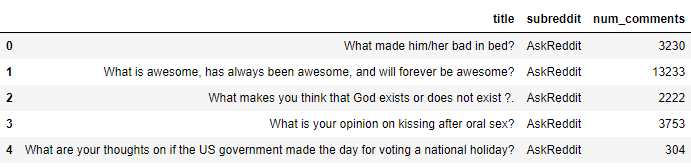
\includegraphics[scale=0.49]{dataframe_posts.png}
    \vspace{-10mm}
    \captionof{figure}{\textbf{Top Posts in r/AskReddit}}
    \vspace{2mm}
    \hspace{5mm}Above is the posts we called through Reddit API. We are planning on as many posts in different subReddits. 
    \vspace{2mm}
    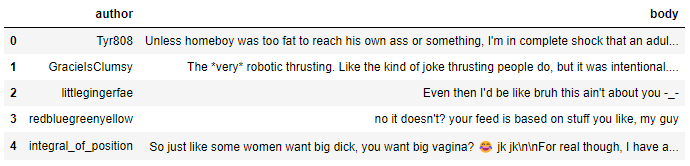
\includegraphics[scale=0.49]{dataframe_comments.png}
    \vspace{-7mm}
    \captionof{figure}{\textbf{Examples of Comments in the Posts of r/AskReddit}}
    \vspace{2mm}
    \hspace{5mm}Above is the example comments of the post written by user name 'ymv4hx' in r/AskReddit. Yet, we are working on the data cleaning process.
\section{Challenges}
    \subsection{Open Challenges and Questions}
    \hspace{5mm}There were so many subReddits, and it was challenging to choose which subReddits to choose, as we want to build an unbiased models.
    
    \subsection{Major Changes}
        \hspace{5mm}No major changes have been made in this week.
\section{Timeline and Roles}
    \subsection{Timeline}
        \begin{tabular}{m{3.8em} | m{19em}} 
        \hline
        Time & Task \\ [0.5ex] 
        \hline\hline
        \small Week 01 & Literature review finish project proposal \\ 
        \hline
        \small Week 02 & Extract data and work on cleaning and organizing it \\
        \hline
        \small Week 03 & Polish classification process and get a final model-tagged data to work with \\
        \hline
        \small Week 04 & Assess model accuracy and start building the network \\
        \hline
        \small Week 05 & Network analysis and visualization \\
        \hline
        \small Week 06 & Compile results and prepare final report \\
        \end{tabular}
    \subsection{Roles}
        \begin{tabular}{m{7.8em} | m{15em}} 
        \hline
        Name & Tasks \\ [0.5ex] 
        \hline\hline
        \small Aviral Chawla & Start building a model for hate speech and find resources regarding a classification model \\ 
        \hline
        \small Daniel Orem & Finalize data cleaning and find resources regarding a classification mode\\
        \hline
        \small Jay Hwasung Jung & Start building a model for hate speech \\
        \hline
        \small Shunsuke Miyazato &  Finalize data cleaning and find resources regarding a classification mode\\
        \end{tabular}
\end{multicols}

\end{document}
